% \section{Experience Lessons learned}
% \begin{enumerate}
% \item engagement is necessary
% \item we must capture all devices, meters, \emph{and} their inter-relationship
% \item we must capture some location and other information about each entity for accounting
% \end{enumerate}

% \section{Challenges: Automation}
% \begin{enumerate}
% \item mobility
% \item bind-dissociation/re-association
% \item energy apportionment/accounting
% \end{enumerate}

\section{Projected results}
\begin{enumerate}
\item audit results
\item energy usage take-aways
\item query time for a typical single-device/lookup query
\item query time for an aggregate query
\end{enumerate}

% \begin{figure}[htb!]
% \begin{center}
% 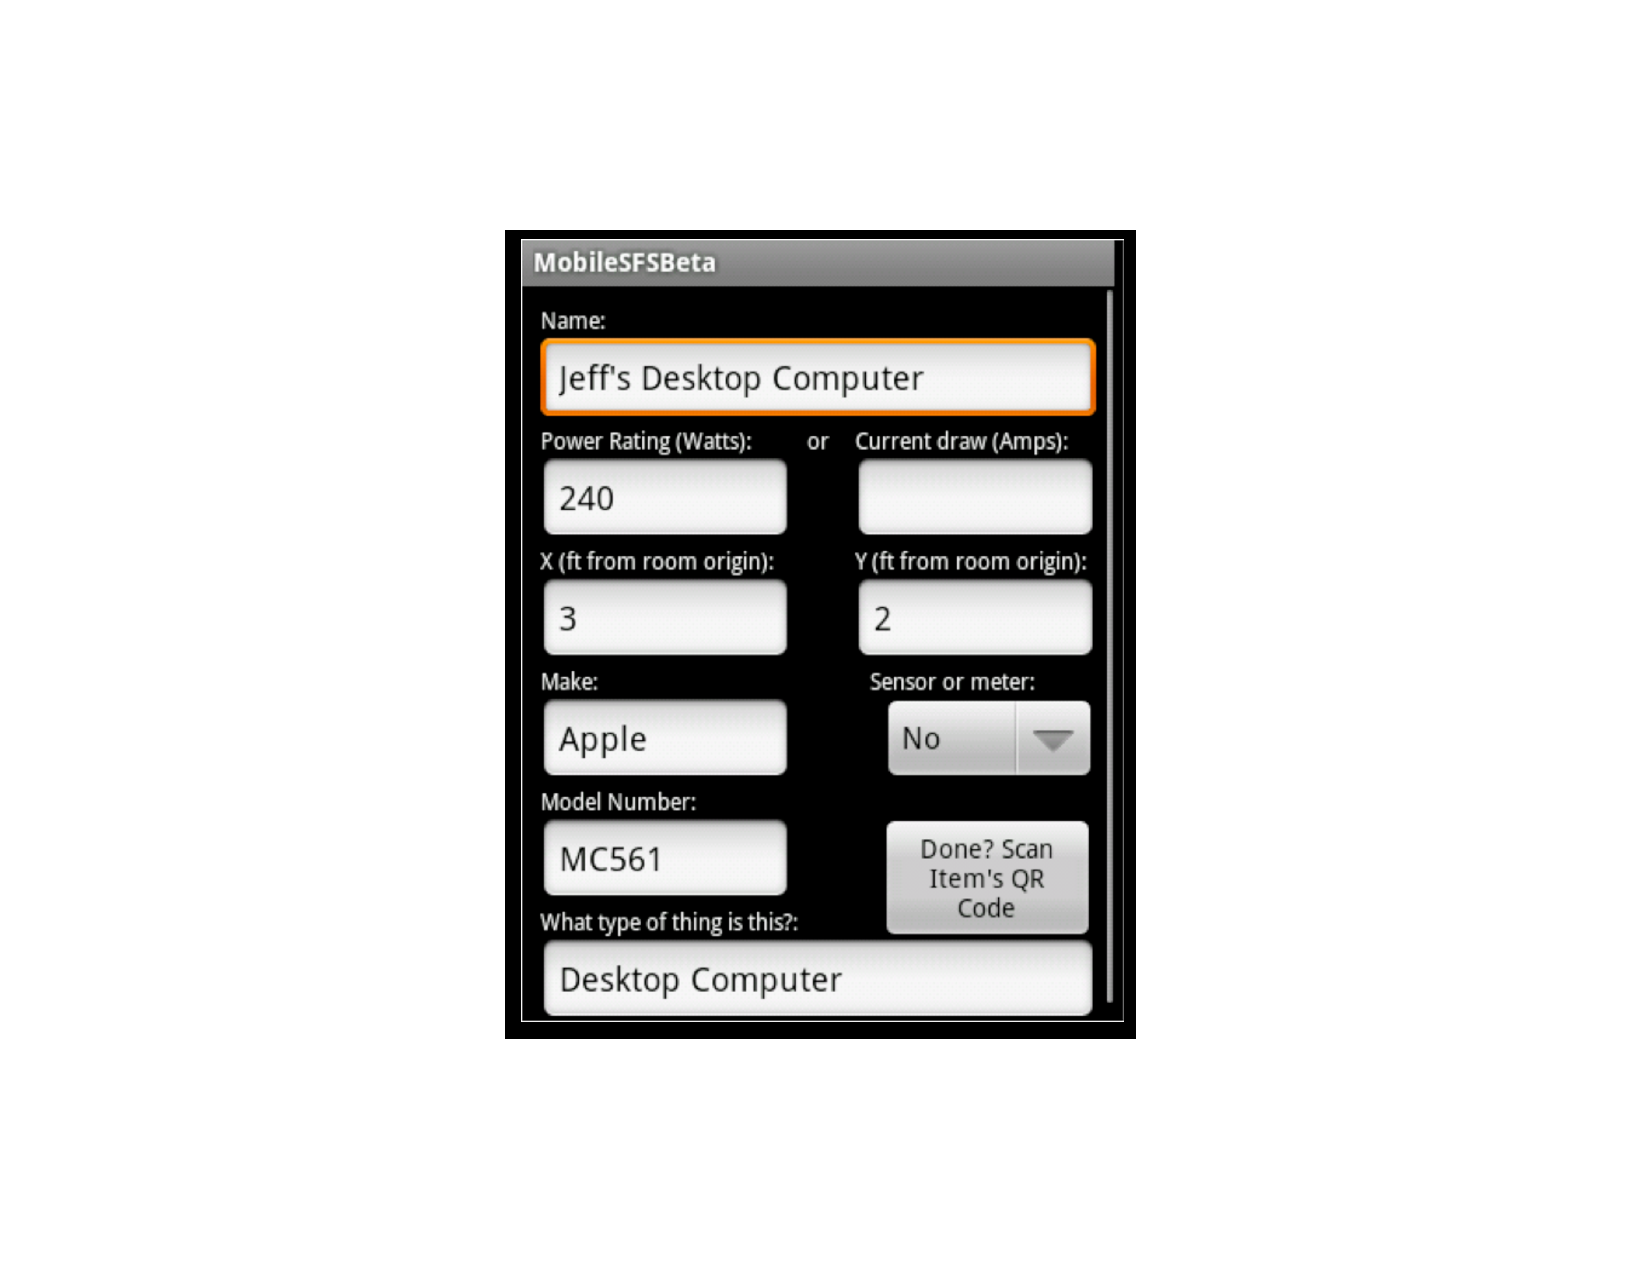
\includegraphics[width=0.8\columnwidth]{figs/screenshot01}
% \caption{The interface presented to the user for entering device and meter information.}
% \label{channelcomp}
% \end{center}
% \end{figure}



\section{Mobile SFS}
\label{sec:mobile}
The phone is the natural point of intersection between the user, the phyiscal world, and virtual services.\\

{\bf Goals}:
\begin{itemize}
\item Personalized energy attribution and tracking
\item Auto-aggregation techniques using stream correlation analysis \\
	\begin{itemize}
	\item identify stream correlations
	\item aggregate according to correlation threshold
	\item at user level, location level, total
	\item dealing with mobility (re-association and aggregation of streams) with dynamic subscriptions
	\end{itemize}
\end{itemize}

{\bf How do we know that the streams being aggregated are the right streams to aggregate?  What's the ground truth?}
Should we ask the user? (this becomes a user study)

The next approach skips this step altogether and establishes \emph{goodness} by comparing before/after aggregate consumption
data for the office.  Does the auto-aggregation help with this at all?

Is this about user engagement or is this about accuracy?  For a systems paper this really should be about accuracy
and should be compared against ground truth.  Ground-truth in this case is user behavior before and user behavior afterwards.


{\bf calibration might be an issue}

\begin{itemize}
\item Items that we were once used together that are no longer used together.
\item Energy consumption per user drops.
\item Cumulative energy consumption drops.
\end{itemize}

{\bf Accounts}:
\begin{itemize}
\item spaces
\item users \\
\end{itemize}

Users use their mobile phone to tag items they are actively using. \\

{\bf Tagging and registration mechanisms}:
\begin{itemize}
\item scan the qr code of the item you are currently using
\item if the item is a shared item, then it can be tagged by multiple users, and the energy can be split amongst all the users
	\begin{itemize}
	\item if a non-personal item is actively being used and nobody claims it, it is charged to all the users that we were in the same space
			as the item when the item became active.
	\item if a non-personal item is actively being used and nobody claims it and nobody was in the space when the item was turned on, it is charged
			to the space.
	\end{itemize}
\item if the item is a single-use item, it can only be used by a single user at time
\item if the item is a personal item, it can only belong to a single user and all energy is charged to that single user \\
\end{itemize}


{\bf Hypotheses}:

\begin{enumerate}
\item Personal energy attribution helps induce changes in behavior that lower energy consumption.
\item Personal energy attribution requires active user participation and engagement.
	\begin{itemize}
	\item Localization can be automated with indoor wifi; lowering participation overhead.
	\end{itemize}
\end{enumerate}



\subsection{Tracking steps}

\begin{enumerate}
\item Bootstrap
\item Tracking
\item Analysis
\item Visualization
\end{enumerate}


\subsubsection{Bootstrap}
The bootstrap phase is step where users become aware that there is energy information out there and it's the essential bootstrapping processes
of getting the user invovled in their energy attribution.  This step consists of:

\begin{enumerate}
\item Tagging items of everyday use with qr codes.
\item Binding meters and items.
\item Tag items as personal, shared, n-multi-shared
\end{enumerate}


All items should be tagged with qr codes.  This involves physically sticking a qr code onto the item, scanning it, and describing the item
that it is attached to.  This should be done for {\bf all items with a measurable energy footprint}, including lights, computers, appliances,
chargers, space heaters, etc.  -- miscenallenous eletrical loads.  A more advanced setup could include eletrical load information or HVAC 
component tagging, if visibility of total energy footprint is of interest.

Binding meters and items is a way of informing the system that the meter serves as an energy-consumption proxy for the item that the meter is
attached to.  This involves scanning both the meter and the item and creating their relationship explicitly.  This allows the application to query
the appropriate meter for historical consumption information when the user wishes to learn about the consumption of the item that is attached to that meter.
This model also assumes that meters are essentially free with respect to energy consumption.  Generally this assumption is not that far from reality.
For example, the ACme~\cite{acme} plugload meter draws on the order of several hundred milliwatts of power versus the tens to hundreds of watts being
consumed by the items it is typically measuring.

Tagging is the final, important step in the engagement phase.  This step requires that user scan items and essentially mark them as personal or shared.
This is used for analytical purposes and attribution.  You cannot determine which account the energy consumption of an item should be debited to without
ownership information.  Our application distinguishes between three types of sharing.  Personal items means that there is an owner relationship between
the item and its owner.  Any energy consumed by the item is attributed to the owner.  Shared items are charged to the user that last made use of the item.
If no user takes ownership of the item it is charged to every user of the system and each user is actively informed of the added charge (discussed in
section~\ref{sec:charge_alerts}).  Finally, the n-multi-shared items are items that can only be shared by N users at any one time.  This feature is essentially
sets an upperbound on the number of accounts that can be chared for the energy consumption of the device.

The cost of engagement is intially high but reduces over time.  The feature that we like best here is that the infrastructure captured through the engagement
step is beneficial for all users in the system and can be constructed iteratively.  The more users you have engaged, the faster the physical infrastructure
can be virtualized.

\subsubsection{Tracking}
%Scan you location/usage.

Tracking is the most active step in the attribution cycle.  This is where the user uses the application to record their location and energy consumption
information.  The infrastructure constructed in the \emph{bootstrap} step allows the user to scan their location and item being used.  For example, when the user walks into a building, she scans the qr code for the building to set their context.  As the user enters their office, they scan the qr code for the office.  Finally, 
before using any electrical device, the user scans it to register it's use.  Personal tags are most useful here, as they reduce this scanning step.
When the user is done using their item, they scan the item again to record that they are no longer using it.

This phase in the processes is the most tedious for the user and we think that more infrastructure and learning can be done to improve tracking.
To minimize interaction we offer mechanisms for grouping usage patterns.  For example, the user can decide to group items into an activity and 
combine streams for items that are associated with that activity.  For instance, each morning a graduate student comes to lab at the same time, 
turns on their PC or laptop, lamp, and prints out some papers.  The student pay group these streams into a single activity which alerts the application
to bin the energy consumed by the associated device to the account belonging to the user.

We also run correlation analysis in the background that looks to associate patterns of usage.  These may be presented to the user for corroboration
and ease the grouping processes.  We discuss its use in section~\ref{sec:correlation_analysis}.

% Analytical triggers

\subsubsection{Analysis}
Using traces generated by user activity, we track their energy usage through detailed accounting.  Our application combines energy consumption data
with contextual streaming data (i.e. location, usage information).  We perform aggregation in time, space, and category per user and group by activity
and location.  We also looks for trends in the data that indicate correlated usage patterns between items and users.  This allows us to ask
the user specific questions about grouping to make out analytics more accurate and reduce the burden imposed on the user during the tracking phase.
It also enables us to present the data to users about correlations amongst one another that could help them plan to use items more efficiently
from an energy perspective.  Details on our analysis is presented in~\ref{sec:analysis_results}.

\subsubsection{Visualization}
Finally, we looks for interesting ways of presenting real-time analytical data to users that could help them understand their own energy usage, as
well as the context of energy usage in their environment.  Our specific aim in this phase is to induce changes in behavior that cause the user to
make better use of their devices and reduce their overall energy consumption.  We demonstrate some of the visualization in section~\ref{sec:viz}
and the overall energy consumption before and after using the application in section~\ref{sec:energy_before_after}.


\section{Results}
This section will go start, first by talking about the overall energy consumption results.  For this, a baseline must be established, either
at the room-aggregate level or the individual user level.  The latter is simpler and is useful for comparing the effect of the system on invidual
energy consumption.  That's really the point of the system.





